\documentclass[12pt]{article}
\setlength{\oddsidemargin}{0in}
\setlength{\evensidemargin}{0in}
\setlength{\textwidth}{6.5in}
\setlength{\parindent}{0in}
\setlength{\parskip}{\baselineskip}

\usepackage{amsmath,amsfonts,amssymb,bm,graphics,pgfplots,framed,dsfont}
\usepackage[scale=0.75,top=1cm,bottom=3cm]{geometry}

\begin{document}

\textbf{Minh Anh Nguyen }\\
\textbf{Calculus 1\hfill }\\
\textbf{Section: 04}\\
\textbf{TA name: Arthur Huey}\\
\noindent\rule{16cm}{0.4pt}

Section 2.1:

\begin{enumerate}
    \setcounter{enumi}{4}

    \item Find an equation of the tangent line to the curve at the given point.
          \begin{center}
              $y = 2x^2 - 5x + 1$\\
              $(3,4)$
          \end{center}
          The slope of the tangent line at (3, 4) is:
          \[ f'(x) = {\displaystyle\lim_{h \to 0} \frac{f(x+h) - f(x)}{h}} \]
          \[ f'(x) = {\displaystyle\lim_{h \to 0} \frac{2(x+h)^2 - 5(x+h) + 1 - 2x^2 + 5x - 1}{h}} \]
          \[ f'(x) = {\displaystyle\lim_{h \to 0} \frac{2x^2 + 4xh + 2h^2 - 5x - 5h - 2x^2 + 5x}{h}} \]
          \[ f'(x) = {\displaystyle\lim_{h \to 0} \frac{4xh + 2h^2 - 5h}{h}} \]
          \[ f'(x) = {\displaystyle\lim_{h \to 0} (4x + 2h - 5)} \]
          \[ m = f'(x) = {\displaystyle 4x} \]
          \[ m = f'(3) = {\displaystyle 4 \times 3} = 12 \]\\
          The equation of the tangent line at (3, 4) is:
          \[y - 4 = 4(x-3)\]
          \[\boxed{y = 4x - 8}\]

          %--%
\end{enumerate}

\newpage

\begin{enumerate}
    \setcounter{enumi}{10}
    \item A cliff diver plunges from a height of $100 ft$ above the water surface. The distance the diver falls in $t$ seconds is given by the function $d(t) = 16t^2 (ft)$.
          \begin{enumerate}
              \item After how many seconds will the diver hit the water? \\
                    The diver hit the water when the distance equals the height above the water surface:
                    \[100 = 16t^2\]
                    \[6.25 = t^2\]
                    \[t = \pm 2.5 \text{ }(second)\]
                    \noindent\fbox{
                        \parbox{380px}{
                            There are no negative time, so the diver will hit the water after 2.5 second.
                        }
                    }
              \item With what velocity does the diver hit the water?\\
                    The equation of the velocity is:
                    \[ d'(t) = \lim_{h \to 0} {\displaystyle \frac{d(t + h) - d(t)}{h}}\]
                    \[ d'(t) = \lim_{h \to 0} {\displaystyle \frac{16(t+h)^2 - 16t^2}{h}}\]
                    \[ d'(t) = \lim_{h \to 0} {\displaystyle \frac{16t^2 + 32th + 16h^2 - 16t^2}{h}}\]
                    \[ d'(t) = \lim_{h \to 0} {\displaystyle \frac{32th + 16h^2}{h}}\]
                    \[ d'(t) = \lim_{h \to 0} {\displaystyle (32t + 6h)}\]
                    \[ d'(t) = 32t \]
                    The diver hit the water after 2.5 second:
                    \[ d'(t) = 32 \time 2.5\]
                    \[\boxed{ d'(t) = 80 (ft/s)}\]
          \end{enumerate}

\end{enumerate}

\begin{enumerate}
    \setcounter{enumi}{16}
    \item For the function $g$ whose graph is given, arrange the following numbers in increasing order and explain your reasoning:
          \[0 \text{ ~~  } g'(-2) \text{  ~~ } g'(0) \text{  ~~ } g'(2) \text{ ~~  } g'(4)\]

          \begin{center}
              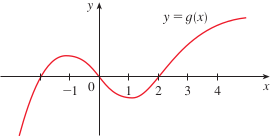
\includegraphics{Images/Image-0.png}
          \end{center}
          Slope of the tangent line are considered as following:\\~\\
          1. Slope at x = -2: The graph is increasing steeply, so the slope is positive and quite large.\\
          2. Slope at x = 0: The graph is decreasing steeply, so the is negative.\\
          3. Slope at x = 2: The graph is increasing steeply, so the slope is positive but it's not as large as x = -2.\\
          4. Slope at x = 4: The graph is increasing gradually, so the slope is positive but it's smaller than x = 2.\\

          Thus the increasing order is:
          \[\boxed{g'(0) \text{ ~~ } 0 \text{ ~~ } g'(4) \text{ ~~ } g'(2) \text{ ~~ } g'(-2)}\]

\end{enumerate}

\begin{enumerate}
    \setcounter{enumi}{18}
    \item The graph of a function $f$ is shown.
          \begin{center}
              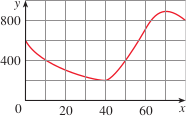
\includegraphics{Images/Image-1.png}
          \end{center}
          \begin{enumerate}
              \item Find the average rate of change of $f$ on the interval $[20, 60]$.\\
                    The average rate of change on the interval $[20, 60]$ is:
                    \[{\displaystyle \frac{f(60) - f(20)}{60 - 20} = \frac{700 - 300}{60 - 20}} = \boxed{100}\]
              \item Identify an interval on which the average rate of change of $f$ is 0.\\
                    An interval on which the average rate of change of $f$ is 0 is $\boxed{[10, 50]}$ because:
                    \[{\displaystyle \frac{f(50) - f(10)}{50 - 10} = \frac{400 - 400}{50 - 210}} = 0\]
              \item Compute and explain what does this value represent geometrically?
                    \[{\displaystyle \frac{f(40) - f(10)}{40-10}} = \boxed{\frac{-200 -400}{40-10} = -200}\]
                    \noindent\fbox{
                        \parbox{380px}{
                            This value represents the average rate of change of $f$ on the interval $[10,40]$.
                        }
                    }
              \item Estimate the value of $f'(50)$.\\
                    The value of $f'(50)$ is approximately equal to the average of change on the interval $[40,60]$:
                    \[f'(50) = {\displaystyle \frac{f(60) - f(40)}{60 - 40} = \frac{700 - 200}{60 - 40}} = \boxed{25}\]
              \item Is $f'(10) > f'(30)$?\\
                    The value of $f'(10)$ is approximately equal to the average of change on the interval $[0,20]$:
                    \[f'(10) = {\displaystyle \frac{f(20) - f(0)}{20 - 0} = \frac{300 - 600}{20 - 0}} = -15\]
                    The value of $f'(30)$ is approximately equal to the average of change on the interval $[20,40]$:
                    \[f'(30) = {\displaystyle \frac{f(40) - f(20)}{40 - 20} = \frac{200 - 300}{40 - 20}} = -5\]
                    \noindent\fbox{
                        \parbox{280px}{
                            Hence, the statement is wrong because $f'(10) < f'(30)$.             }
                    }
              \item Is $f'(60) > {\displaystyle \frac{f(80) - f(40)}{80-40}}$? Explain.\\~\\
                    The value of $f'(60)$ is approximately equal to the average of change on the interval $[50,70]$:
                    \[f'(60) = {\displaystyle \frac{f(70) - f(50)}{70 - 50} = \frac{900 - 400}{70 - 50}} = 25\]
                    \[{\displaystyle \frac{f(80) - f(40)}{80-40}} = \frac{800 - 200}{80-40} = 15\]
                    \noindent\fbox{
                        \parbox{160px}{
                            Hence, the statement is correct.
                        }
                    }
          \end{enumerate}

\end{enumerate}

\begin{enumerate}
    \setcounter{enumi}{20}
    \item Use Equation 5 to find $f'(a)$ at the given number $a$.\\
          \[f(x) = {\displaystyle \frac{x^2}{x+6}}, a = 3\]
          \[f'(a) = {\displaystyle \lim_{x \to a} \frac{f(x) - f(a)}{x - a}}\]
          \[f'(a) = {\displaystyle \lim_{x \to a} \frac{\frac{x^2}{x + 6} - \frac{a^2}{a + 6}}{x - a}}\]
          \[f'(a) = {\displaystyle \lim_{x \to a} \frac{\frac{x^2(a+6) - a^2(x+6)}{(x+6)(a+6)}}{x - a}}\]
          \[f'(a) = {\displaystyle \lim_{x \to a} \frac{x^2a + 6x^2 - a^2x - 6a^2}{(x - a)(x+6)(a+6)}}\]
          \[f'(a) = {\displaystyle \lim_{x \to a} \frac{x^2a - a^2x + 6x^2 - 6a^2}{(x - a)(x+6)(a+6)}}\]
          \[f'(a) = {\displaystyle \lim_{x \to a} \frac{xa(x - a) + 6(x^2 - a^2)}{(x - a)(x+6)(a+6)}}\]
          \[f'(a) = {\displaystyle \lim_{x \to a} \frac{xa(x - a) + 6(x - a)(x+a)}{(x - a)(x+6)(a+6)}}\]
          \[f'(a) = {\displaystyle \lim_{x \to a} \frac{(x - a)(xa + 6x + 6a)}{(x - a)(x+6)(a+6)}}\]
          \[f'(a) = {\displaystyle \lim_{x \to a} \frac{(xa + 6x + 6a)}{(x+6)(a+6)}}\]
          \[f'(a) = {\displaystyle \frac{(a^2 + 6a + 6a)}{(a+6)(a+6)}}\]
          \[f'(a) = {\displaystyle \frac{(a^2 + 12a)}{(a+6)^2}}\]
          \[f'(3) = {\displaystyle \frac{(3^2 + 12\times3)}{(3+6)^2}} = \boxed{\frac{5}{9}}\]
\end{enumerate}

\begin{enumerate}
    \setcounter{enumi}{22}
    \item Find $f'(a)$.
          \[f(x) = 2x^2 - 5x + 3\]
          \[f'(a) = \lim_{x \to a} \frac{f(x) - f(a)}{x - a} \]
          \[f'(a) = \lim_{x \to a} \frac{2x^2 - 5x + 3 - 2a^2 + 5a - 3}{x - a} \]
          \[f'(a) = \lim_{x \to a} \frac{2x^2 - 2a^2 - 5x + 5a}{x - a} \]
          \[f'(a) = \lim_{x \to a} \frac{2(x^2 - a^2) - 5(x - a)}{x - a} \]
          \[f'(a) = \lim_{x \to a} \frac{2(x - a)(x + a) - 5(x - a)}{x - a} \]
          \[f'(a) = \lim_{x \to a} \frac{(x - a)(2x + 2a - 5)}{x - a} \]
          \[f'(a) = \lim_{x \to a} (2x + 2a - 5) \]
          \[f'(a) = 2a + 2a - 5 \]
          \[\boxed{f'(a) = 4a - 5}\]
\end{enumerate}

\begin{enumerate}
    \setcounter{enumi}{28}
    \item If $f(x) = 3x^2 - x^3$, find $f'(1)$ and use it to find an equation of the tangent line to the curve $y = 3x^2 - x^3$ at the point (1, 2).\\
          \[f'(a) = {\displaystyle \lim_{h \to 0} \frac{f(a+h) - f(a)}{h}}\]
          \[f'(a) = {\displaystyle \lim_{h \to 0} \frac{3(a+h)^2 - (a+h)^3 - 3a^2 + a^3}{h}}\]
          \[f'(a) = {\displaystyle \lim_{h \to 0} \frac{3a^2 + 6ah + 3h^2 - a^3 - 3a^2h - 3ah^2 - h^3 - 3a^2 + a^3}{h}}\]
          \[f'(a) = {\displaystyle \lim_{h \to 0} \frac{6ah + 3h^2 - 3a^2h - 3ah^2 - h^3}{h}}\]
          \[f'(a) = {\displaystyle \lim_{h \to 0} (6a + 3h - 3a^2 - 3ah - h^2)}\]
          \[f'(a) = {\displaystyle \lim_{h \to 0} (6a + 3h - 3a^2 - 3ah - h^2)}\]
          \[f'(a) = {\displaystyle 6a - 3a^2}\]
          \[f'(1) = {\displaystyle 6 \times 1 - 3 \times 1^2} = 3\]
          Equation of the tangent line is:
          \[y - 2 = 3(x - 1)\]
          \[\boxed{y = 3x -1}\]
\end{enumerate}

\begin{enumerate}
    \setcounter{enumi}{42}
    \item Each limit represents the derivative of some function $f$ at some number $a$. State such an $f$ and $a$ in each case.\\
          \[{\displaystyle \lim_{h \to 0} \frac{\sqrt{9+h} - 3}{h}}\]
          \[\boxed{f(x) = \sqrt{x}, \text{~ } a = 9}\]

\end{enumerate}

\newpage

Section 2.2:
\begin{enumerate}
    \setcounter{enumi}{6}
    \item Trace or copy the graph of the given function $f$. (Assume that the axes have equal scales.) Then use the method of Example 1 to sketch the graph of $f'$ below it.
          \begin{center}
              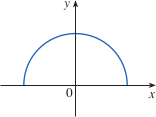
\includegraphics{Images/Image-2.png}
          \end{center}
          \begin{figure}[!h]
              \begin{framed}
                  \centering
                  \begin{tikzpicture}
                      \begin{axis}[
                              axis lines = center,
                              xmin=-5,xmax=5,
                              ymin=-7,ymax=7,
                              yticklabels=\empty,
                              xticklabels=\empty,
                          ]
                          \addplot [
                              domain=-8:8,
                              samples=100,
                              color=red,
                          ]
                          {(-2*x)/(sqrt(4-x^2))};
                      \end{axis}
                  \end{tikzpicture}
              \end{framed}
          \end{figure}
\end{enumerate}

\newpage

\begin{enumerate}
    \setcounter{enumi}{11}
    \item Shown is the graph of the population function $P(t)$ for yeast cells in a laboratory culture. Use the method of Example 1 to graph the derivative $P'(t)$. What does the graph of $P'$ tell us about the yeast population?
          \begin{center}
              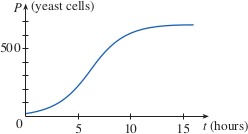
\includegraphics{Images/Image-3.png}
          \end{center}
          \begin{figure}[!h]
              \begin{framed}
                  \centering
                  \begin{tikzpicture}
                      \begin{axis}[
                              axis lines = left,
                              xmin=-0.85,xmax=5,
                              ymin=-7,ymax=7,
                              yticklabels=\empty,
                              xticklabels=\empty,
                          ]
                          \addplot [
                              domain=-8:8,
                              samples=100,
                              color=red,
                          ]
                          {-4*x^2 + 5*x};
                      \end{axis}
                  \end{tikzpicture}
              \end{framed}
          \end{figure}

          \noindent\fbox{
              \parbox{390px}{
                  The yeast population will grow rapidly at first, but will slow down over time.
              }
          }
\end{enumerate}

\begin{enumerate}
    \setcounter{enumi}{24}
    \item Find the derivative of the function using the definition of derivative. State the domain of the function and the domain of its derivative.
          \[f(x) = {\displaystyle \frac{1}{x^2-4}}\]
          The domain of $f(x)$ is:
          \[x^2 - 4 \neq 0\]
          \[x \neq \pm 2\]
          Hence, the domain of $f(x)$ is: $\boxed{\mathds{R} \setminus \{-2,2\}}$\\
          The derivative of $f(x)$ is:
          \[f'(x) = {\displaystyle \lim_{h \to 0} \frac{f(x+h) - f(x)}{h}}\]
          \[f'(x) = {\displaystyle \lim_{h \to 0} \frac{\frac{1}{(x+h)^2-4} - \frac{1}{x^2-4}}{h}}\]
          \[f'(x) = {\displaystyle \lim_{h \to 0} \frac{\frac{1}{x^2+xh+h^2-4} - \frac{1}{x^2-4}}{h}}\]
          \[f'(x) = {\displaystyle \lim_{h \to 0} \frac{x^2-4-x^2-xh-h^2+4}{h(x^2+xh+h^2-4)(x^2-4)}}\]
          \[f'(x) = {\displaystyle \lim_{h \to 0} \frac{-xh-h^2}{h(x^2+xh+h^2-4)(x^2-4)}}\]
          \[f'(x) = {\displaystyle \lim_{h \to 0} \frac{-x-h}{(x^2+xh+h^2-4)(x^2-4)}}\]
          \[f'(x) = {\displaystyle \frac{-x}{(x^2-4)(x^2-4)}}\]
          \[\boxed{f'(x) = {\displaystyle \frac{-x}{(x^2-4)^2}}}\]
          The domain of $f'(x)$ is:
          \[(x^2 - 4)^2 \neq 0\]
          \[x^2 - 4 \neq 0\]
          \[x \neq \pm 2\]
          Hence, the domain of $f'(x)$ is: $\boxed{\mathds{R} \setminus \{-2,2\}}$\\

\end{enumerate}

\begin{enumerate}
    \setcounter{enumi}{30}
    \item Sketch the graph of $f(x) = 1 + \sqrt{x+3}$ by starting with the graph of $y = \sqrt{x}$ and using the transformations of Section 1.3.

          First, we draw $f(x) = \sqrt{x}$.

          \begin{figure}[!h]
              \centering
              \begin{tikzpicture}
                  \begin{axis}[
                          axis lines = center,
                          xlabel = \(x\),
                          ylabel = {\(f(x)\)},
                          xmin=-10, xmax=10,
                          ymin=-2, ymax=2,
                      ]
                      \addplot [
                          domain=0:10,
                          samples=100,
                          color=red,
                      ]
                      {sqrt(x)};
                  \end{axis}
              \end{tikzpicture}
          \end{figure}
          \newpage
          And then, we draw $f(x + 3)$:
          \begin{figure}[!h]
              \centering
              \begin{tikzpicture}
                  \begin{axis}[
                          axis lines = center,
                          xlabel = \(x\),
                          ylabel = {\(f(x)\)},
                          xmin=-10, xmax=10,
                          ymin=-2, ymax=2,
                      ]
                      \addplot [
                          domain=-3:10,
                          samples=100,
                          color=red,
                      ]
                      {sqrt(x+3)};
                  \end{axis}
              \end{tikzpicture}
          \end{figure}

          Finally, we draw $f(x+3) + 1$.

          \begin{figure}[!h]
              \begin{framed}
                  \centering
                  \centering
                  \begin{tikzpicture}
                      \begin{axis}[
                              axis lines = center,
                              xlabel = \(x\),
                              ylabel = {\(f(x)\)},
                              xmin=-10, xmax=10,
                              ymin=-2, ymax=2,
                          ]
                          \addplot [
                              domain=0:10,
                              samples=100,
                              color=red,
                          ]
                          {sqrt(x)};
                      \end{axis}
                  \end{tikzpicture}
              \end{framed}
          \end{figure}

\end{enumerate}

\begin{enumerate}
    \setcounter{enumi}{36}
    \item Let $P$ represent the percentage of a city’s electrical power that is produced by solar panels $t$ years after January 1, 2020.
          \begin{enumerate}
              \item What does $dP/dt$ represent in this context?\\~\\
                    \noindent\fbox{
                        \parbox{410px}{
                            $dP/dt$ is the rates of change of the percentage $P$ of a city’s electrical power with respect to $t$ years.
                        }
                    }\\
              \item Interpret the statement
                    \[ \left. \begin{array}{l}
                            \frac{dP}{dt}\end{array} \right|_{t-2} = 3.5  \]
                    \noindent\fbox{
                        \parbox{410px}{
                            On January 2018, the rates of increasing of the percentage of a city's electrical power is $3.5 (\%)$.
                        }
                    }\\
          \end{enumerate}
\end{enumerate}

\begin{enumerate}
    \setcounter{enumi}{54}
    \item Let $f(x) = \sqrt[3]{x}$.
          \begin{enumerate}
              \item If $a \neq 0$, use Equation 2.1.5 to find $f'(a)$.
                    \[f'(a) = {\displaystyle \lim_{x \to a} \frac{f(x) - f(a)}{x-a}}\]
                    \[f'(a) = {\displaystyle \lim_{x \to a} \frac{\sqrt[3]{x} - \sqrt[3]{a}}{x-a}}\]
                    \[f'(a) = {\displaystyle \lim_{x \to a} \frac{(\sqrt[3]{x} - \sqrt[3]{a})(\sqrt[3]{x}^2 + \sqrt[3]{a}^2 + \sqrt[3]{ax})}{(x-a)(\sqrt[3]{x}^2 + \sqrt[3]{a} + \sqrt[3]{ax})}}\]
                    \[f'(a) = {\displaystyle \lim_{x \to a} \frac{x-a}{(x-a)(\sqrt[3]{x}^2 + \sqrt[3]{a}^2 + \sqrt[3]{ax})}}\]
                    \[f'(a) = {\displaystyle \lim_{x \to a} \frac{1}{(\sqrt[3]{x}^2 + \sqrt[3]{a}^2 + \sqrt[3]{ax})}}\]
                    \[f'(a) = {\displaystyle \frac{1}{(\sqrt[3]{a}^2 + \sqrt[3]{a}^2 + \sqrt[3]{a}^2)}}\]
                    \[\boxed{f'(a) = {\displaystyle \frac{1}{3\sqrt[3]{a}^2}}}\]
              \item Show that $f'(0)$ does not exist.
                    \[f'(0) = {\displaystyle \frac{1}{3\sqrt[3]{0}^2}}\]
                    \[f'(0) = {\displaystyle \frac{1}{0}}\]
                    \noindent\fbox{
                        \parbox{270px}{
                            Because we cannot divide by 0, $f'(0)$ does not exist.
                        }
                    }\\
              \item Show that $y = \sqrt[3]{x}$ has a vertical tangent line at (0,0). (Recall the shape of the graph $f$. See Figure 1.2.13.)\\
                    The slope of the tangent line at (0,0) is:
                    \[f'(0) = {\displaystyle \frac{1}{0}}\]

                    \noindent\fbox{
                        \parbox{410px}{
                            Because the slope of the tangent line approachs infinity as x approachs 0, we can conclude that there is a vertical tangent line at (0, 0).
                        }
                    }\\
          \end{enumerate}
\end{enumerate}

\end{document}
